\documentclass[10pt]{article}

%\usepackage{hyperref}
\usepackage{natbib}
\usepackage{graphicx}
\usepackage{url}
\usepackage{fancyhdr}
\usepackage{trust}
\pagestyle{fancy}

\lhead{}
\rhead{}
%%\chead{\bfseries U.S. Government Proprietary, For Official Use Only}
\lfoot{\copyright The University of Kansas, 2012}
\cfoot{\thepage}


\newtheorem{conjecture}{Conjecture}
\newtheorem{obligation}{Obligation}
\newtheorem{definition}{Definition}


\usepackage{ifthen}
\newboolean{submission}  %%set to true for the submission version
\setboolean{submission}{false}
%\setboolean{submission}{true}
\ifthenelse
{\boolean{submission}}
{ \newcommand{\todo}[1]{ } } % hide todo
{ \newcommand{\todo}[1]{ % show todo
   \marginpar{\raggedright\footnotesize{#1}}
               }}

\parskip=\medskipamount
\parindent=0pt

\bibliographystyle{abbrvnat}

\title{TPM Specification Design}
\author{Perry Alexander \and Brigid Halling}

\begin{document}

\maketitle
\tableofcontents
\listoffigures
\listoftables

\begin{abstract}
  The abstract goes here...
\end{abstract}

\section{Introduction}

\section{Modeling Approach}

\section{Verification Approach}

The approach taken for verification is establishing a \emph{weak
  bisimulation}~\citep{Sangiorgi:12:Introduction-to} relation between
an abstract requirements model and a model derived from the TPM
specification as shown in figure~\ref{fig:bisimulation}.

\begin{figure}[hbtp]
  \centering
  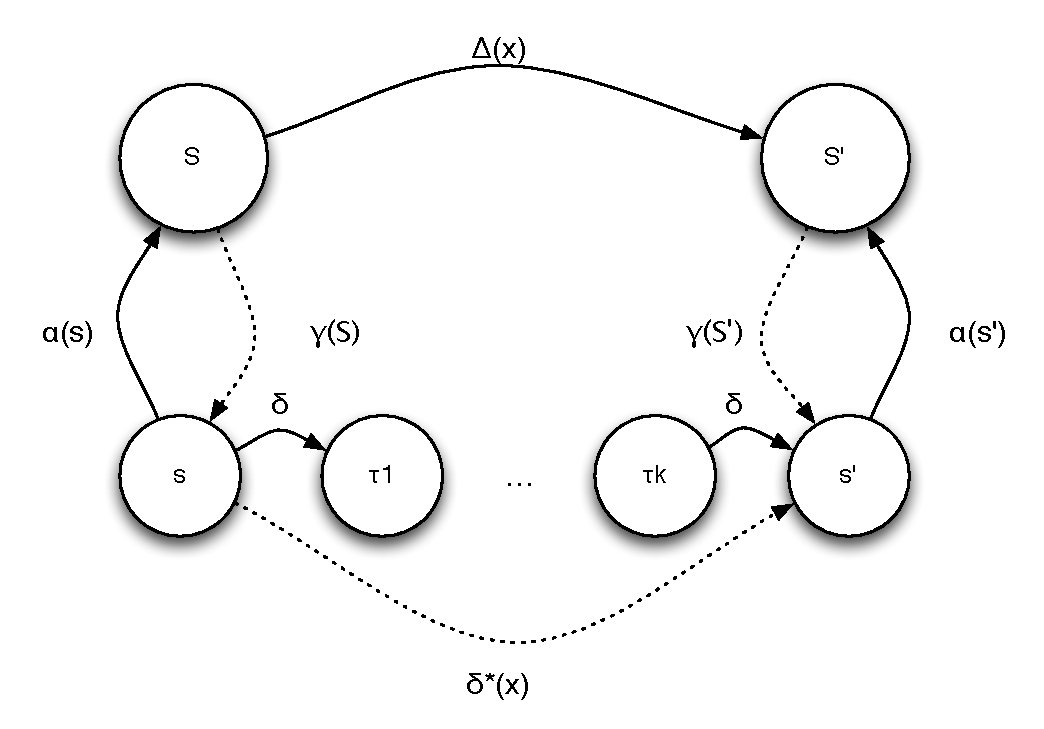
\includegraphics[width=0.75\textwidth]{figures/bisimulation.pdf}
  \caption{Weak bisimulation relation between an abstract transition
    system $A=(S,\Sigma,\Delta)$ and a concrete transition system
    $C=(s,\sigma,\delta)$.}
  \label{fig:bisimulation} 
\end{figure}

We say that $A=(S,\Sigma,\Delta)$ is an \emph{abstract model} where
$S$ is a set of abstract states, $\Sigma$ is a set of actions on
states and input, and $\Delta : S\times\Sigma\rightarrow\Sigma$ is a
transitions on state and action.  Similarly, we say that
$C=(s,\sigma,\delta)$ is a \emph{concrete state } where $s$ is a set
of concrete states, $\sigma$ is a set of actions on states and input,
and $\delta : s\times\sigma\rightarrow\sigma$ is a transition
function.

We relate the abstract and concrete models through an \emph{abstraction
function}, $\alpha:s\rightarrow S$, and \emph{concretization
function}, $\gamma:S\rightarrow 2^s$.  The abstraction and
concretization functions must form a Galois Connection such that:

\[s\in\gamma(\alpha(s))\]

\noindent Specifically, when making the result of an abstraction
concrete, the original state must be in the resulting set.  Note that
the concretization function may result in multiple states due to the
necessity of specifying unknown detail.

We say that $A$ and $C$ are weakly bisimilar ($A\sim C$) if when
$\alpha(s)=S$ then $\alpha(\delta^*(s))=\Delta(S)$ for all inputs to
$s$.

\begin{definition} 
  \[A\sim C \equiv \forall s_0:s \cdot \exists S_0:S \cdot
  \alpha(s_0)=S_0 \Rightarrow \alpha(\delta^*(s_0))=\Delta(S_0)\]
  \label{def:bisimulation}
\end{definition}

In the formal TPM model \texttt{tpmAbsState} defines $S$ while
\texttt{tpmConcState} defines $s$.

\appendix

\chapter{Glossary}
\label{chapt:glossary}

This glossary is intended to document some common acronyms as well as
define some common terms.  It is currently a bit haphazard and a
number of elements are missing.

\section{Trusted Platform Definitions}

\begin{description}
  \parskip=0pt
  \itemsep=\smallskipamount
\item[Trusted Platform Module (TPM)] -- Hardware Trusted Platform
  Module as defined by TCG.
\item[Process Configuration Register (PCR)] -- Registers defined in
  the TPM.  In the TPM there are at least 16 and they are 20 bytes
  wide.
\item[Bound to PCR] -- Encryption including PCR values that must match
  TPM PCR values before decryption is performed.
\item[Sealed to State] -- Operation performed by the TPM where data is
  encrypted and bound to PCRs or a PCR composite that must be checked
  before unsealing.  Only data is sealed.
\item[Wrapped Key] -- An asymmetric key with its private key encrypted
  and its public key visible.  Only keys are wrapped.
\item[Virtual TPM (vTPM)] -- A virtual Trusted Platform Module
\item[Certified Key (CK)] - Asymmetric key with private key signed by the
  AIK private key.
\item[Endorsement Key (EK)] - Asymmetric key who's private key is in
  the TPM hardware.  Private key is used to sign data from TPM while
  public key is used to encrypt sensitive data sent to the TPM.  The
  EK is set by the TPM factory and may not be reset.
\item[Attestation Identity Key (AIK)] - Asymmetric key whose private
  key is used for only two purposes: (i) sign (or attest to) TPM
  internal state; (ii) sign (or certify) other general purpose keys.
  AIKs are generated by a TPM, certified by a trusted third party,
  and used for signing in lieu of the EK.
\item[Storage Root Key (SRK)] - Root of secure storage hierarchy.
  Used to encrypt storage keys that exist outside the TPM.  The SRK
  may be reset.
\item[Attestation Identity Certificate (AIC)] - Certificate
  provided by a trusted third party binding an AIK to a specific
  trusted platform.
\item[Digest] - 20-byte Value contained in a PCR.
\item[PCR Composite] - Single digest value generated from a collection
  of PCR values.
\item[Quote] - A value along with a set of PCR values or PCR composite
  signed by a TPM using an AIK.
\item[Root of Trust for Measurement (RTM)] - the ``place to stand''
  for measurement.  Effectively a hardware-based trusted launch point
  that will faithfully measure, start and pass control to its target
  without trusting other components.
\item[Root of Trust for Storage (RTS)] - the ``place to stand'' for
  measurement storage.  Effectively a trusted hardware store that will
  store measurements with integrity without trusting other components.
\item[Root of Trust for Reporting (RTR)] - the ``place to stand'' for
  generating quotes and providing evidence with integrity and
  authenticity.  Effectively a trusted hardware component that
  generates and signs quotes.
\end{description}

\section{Cryptography Notations}

\begin{description}
  \itemsep=0pt
  \parskip=\smallskipamount
\item[Hash Notation] $\hash{data}$ - The hash of $data$.
\item[Certificate Notation] $\cert{cert}{key}$ - Certificate, $cert$, signed by
  $key$.
\item[Signed Data Notation] $\sign{data}{key}$ - $data$, signed by $key$.
\item[Encrypted Data Notation] $\encrypt{data}{key}$ - $data$
  encrypted with $key$.
\item[Sealed Data Notation] $\seal{data}{pcrs}$ - $data$ sealed to
  $pcrs$.
\item[Wrapped Key Notation] $\wrap{k}{pcrs}$ - Equivalent to the key
  pair $(\seal{\private{k}}{pcrs},\public{k})$
\end{description}

\section{Intel Secure Boot}

\begin{description}
  \itemsep=0pt
  \parskip=\smallskipamount
\item[Trusted eXecution Technology (TXT)] - Intel's trusted boot
  support.
\item[Measured Launch Environment (MLE)] - Run time environment
  providing a measured boot.  Initialized and started by the SINIT
  command execution.
\item[SENTER or GETSEC] - Intel's trusted boot command.  Provides
  synchronization, special bus cycles, and a special environment
  residing on the CPU (ACEA).
\item[Secure INITialization Instructions (SINIT)] - Code for
  performing secure initialization.  Loaded by SENTER and validated by
  the ACM.
\item[Authenticated Code Execution Area (ACEA)] - CPU resident
  environment for executing code known as the Authenticated Code
  Module (ACM).  Boot sequence involving SENTER and SINIT is as
  follows:

  \begin{enumerate}
    \parskip=0pt\itemsep=0pt
  \item Load SINIT and MLE into memory
  \item Invoke SENTER (GETSEC)
  \item Establish special environment (ACEA)
  \item Load SINIT into ACEA
  \item Validate SINIT digital signature and store SINIT identity in
    TPM
  \item SINIT measures MLE in memory and stores MLE identity in TPM
  \item SINIT passes control to MLE
  \end{enumerate}

\item[Authenticated Code Module (ACM)] - Code running in the ACEA. May
  be used for validating platform configuration, measuring the
  measured launch environment, cleaning up after crashes.
\end{description}



%%\nocite{}

\bibliography{tpm-spec-design}

\end{document}
